% Journal of Bioinformatics and Computational Biology submission source.
% Uses the unmodified author-supplied World Scientific class dated 2026/05/18.
\pdfminorversion=7
\pdfsuppresswarningpagegroup=1
\documentclass{ws-jbcb}
\setlength{\paperheight}{11in}

\usepackage[super]{cite}
\usepackage{xcolor}
\usepackage[verbose,hypertexnames=false]{hyperref}
\hypersetup{colorlinks=false,allbordercolors=blue,pdfborderstyle={/S/U/W 1}}
\usepackage{array}
\usepackage{tabularx}
\usepackage{xurl}

\graphicspath{{./}}

% theorem, proposition, definition, example, remark, and proof are class-native.
\newtheorem{algorithm}{Algorithm}
\numberwithin{equation}{section}

\newcommand{\tas}{\textit{Arabidopsis thaliana}}
\newcommand{\ath}{\textit{A.\ thaliana}}
\newcommand{\hs}{\textit{Homo sapiens}}
\newcommand{\TAU}{\tau}
\newcommand{\xRightarrow}[1]{\stackrel{#1}{\Longrightarrow}}
\newcommand{\LTS}{\mathcal{L}}
\newcommand{\powerset}{\mathcal{P}}
\newcommand{\strongsim}{\mathrel{\sim_{s}}}
\newcommand{\weaksim}{\mathrel{\sim_{w}}}
\newcommand{\weakpre}{\mathrel{\preceq_{w}}}
\newcolumntype{Y}{>{\raggedright\arraybackslash}X}

\hypersetup{
  pdftitle={Locating resolution-dependent behavioral correspondence in qualitative DNA-damage response models},
  pdfauthor={Carlos Ramirez Ovalle},
  pdfkeywords={DNA-damage response, observational resolution, qualitative biological networks, model comparison, Petri nets, weak bisimulation}
}

\begin{document}

\markboth{C. Ramirez Ovalle}{Resolution-dependent correspondence in DNA-damage models}
\catchline{}{}{}{}{}

\title{Locating resolution-dependent behavioral correspondence in qualitative DNA-damage response models}

\author{Carlos Ramirez Ovalle\footnote{Corresponding author.}}

\address{Department of Natural Sciences and Mathematics, Pontificia Universidad
Javeriana Cali, Calle 18 No. 118-250, Via a Pance, Cali, Valle del Cauca,
Colombia\\
carlosovalle@javerianacali.edu.co}

\maketitle

\begin{abstract}
Qualitative DNA-damage response models can share functional organization while
encoding different regulatory and terminal mechanisms. Their correspondence
therefore depends on which biological events a comparison observes. We ask at
what declared resolution curated animal/human and \textit{Arabidopsis} models
cease to support matching damage-response choices. We construct finite
executable transition systems from the models and compare their recursive
branching under three literature-motivated observational interfaces. The two
unchanged Petri-net structures have PN-GDDA similarity 0.9976. At coarse
functional and pathway-level resolution, the models match each other's
observable steps and choices after internal events are hidden: they are weakly
bisimilar. Distinguishing mammalian apoptosis from the encoded plant SMR and
differentiation/endoreduplication sequence eliminates both simulation directions,
while structural similarity remains constant. This comparison locates a
compatibility boundary within the declared interfaces, rather than discovering
the already encoded mechanistic differences. Formal decisions are supported by
proofs and independent computational checks. The result shows how readout
selection changes conclusions about these executable models; it does not
establish organism-level equivalence or an experimentally validated
cross-species boundary.

\end{abstract}

\keywords{DNA-damage response; observational resolution; qualitative biological networks; model comparison; Petri nets; weak bisimulation.}

\section{Introduction}\label{sec:introduction}

Qualitative network models make biological hypotheses executable without
requiring a fully parameterized kinetic description. Models assembled for
related functions may nevertheless differ in organism, curation, initial
condition, or update convention. For computational biology, comparing them
requires more than recognizing similar wiring: one must ask whether the models
can reproduce the same biologically relevant steps and choices under a stated
readout.\cite{ChaouiyaPetriBio2007,Li2006,Fisher2007}

DNA-damage response provides a concrete example. Animal/human and
\tas{} models share lesion detection, checkpoint activation, repair, and
recovery, but encode different regulatory and terminal responses. Mammalian
p53-associated control and apoptosis are not the plant-specific SOG1 network,
SMR-associated arrest, or damage-induced differentiation/endoreduplication.
These distinctions are supported independently of our comparison by DDR
literature.\cite{JacksonBartek2009,BlackfordJackson2017,Yoshiyama2013,
DeSchutter2007,Yi2014,Adachi2011} Asking simply whether the models are
``similar'' conceals the choice of biological resolution. We instead ask:
\emph{at which declared observational resolution do their encoded
damage-response choices cease to correspond?}

A structural comparator such as PN-GDDA characterizes local Petri-net wiring,
not transition labels, the initial marking, hidden events, or recursive
reachable choices.\cite{Szawulak2022} Linear event sequences add order but
still do not specify when a choice becomes committed. A model that commits
early to one of two outcomes can have the same sequences as a model that keeps
both outcomes available longer, yet fail to reproduce the latter's branching
options. This matters when a model comparison is intended to preserve choices,
not merely lists of possible endpoints.

Our computational approach first declares what the biological readout can
distinguish. We then construct the finite executable states and ask whether
each observed step can be matched while preserving that ability at the
resulting state pair. Matching in both directions using one consistent relation
is weak bisimulation; matching in one direction is weak simulation. Internal
events are ignored only when the declared interface makes them unobservable.
These standard relations\cite{Milner1989,Sangiorgi2011} supply a
branching-sensitive model comparison, rather than a new biological similarity
score. For models $N_1,N_2$ and observational interface $\Sigma$,
\begin{equation}\label{eq:comparison-map}
 (N_1,N_2,\Sigma)\longmapsto(\LTS(N_1),\LTS(N_2))
 \longmapsto C_\Sigma(\LTS(N_1),\LTS(N_2)),
\end{equation}
where $\LTS(N_i)$ is the reachable labeled transition system and $C_\Sigma$
reports the strongest supported relation. The biological question and the
observational resolution precede that calculation (Fig.~\ref{fig:pipeline}).

The principal result concerns the curated GIM (genome-instability/DNA-repair)
pair. Its unchanged structures score 0.9976 by PN-GDDA, yet the behavioral
answer changes across three declared interfaces. Coarse functional and
pathway-resolved observations retain weak bisimilarity. Exposing distinct
terminal mechanisms makes the models non-comparable in both directions. The
useful output is the location of this change within the tested interfaces,
not the rediscovery of the mechanistic differences already encoded in them.

The contributions are a resolution-specific comparison question, its executable
GIM demonstration, a branching-sensitive computational method with explicit
orientation, and independent formal/software checks supporting that method.
Secondary curated comparisons illustrate one-way matching; an exploratory
HPN-DREAM/CASPOTS analysis confronts model relations with held-out response
data.\cite{Hill2016,Razzaq2018} The study does not establish organism-level
equivalence, experimental validation of the GIM boundary, or predictive
discrimination. It distinguishes the biological knowledge used to construct
interfaces from the model-dependent relationship computed under them.

\begin{figure}[t]
\centering
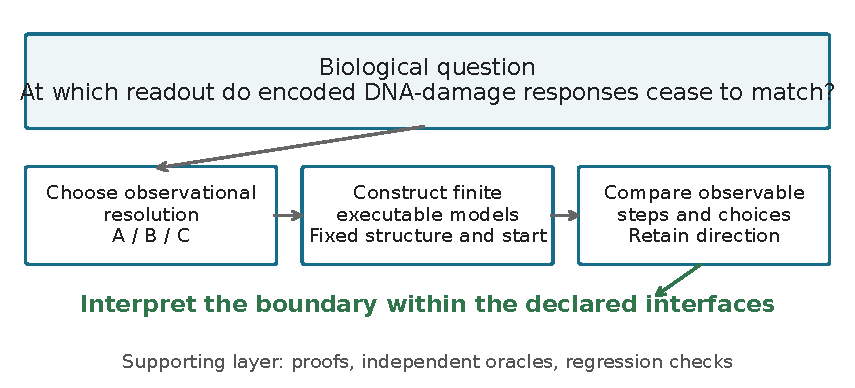
\includegraphics[width=\textwidth]{R2_Fig1.pdf}
\caption{Question-first comparison workflow. Biological readout selection
determines the observational interface before executable models are compared.
Formal verification supports the computation; the endpoint is an explicitly
model-conditional interpretation of the compatibility boundary.}
\label{fig:pipeline}
\alttext{A biological comparison question leads to readout selection, executable
models, branching comparison, and interpretation, with verification below.}
\end{figure}

\section{Biological comparison problem and models}
\label{sec:applications}

\subsection{Biological question and observational-interface principles}
\label{sec:gim-question}

The central question is whether the animal/human and \tas{} DNA-damage models
encode a common executable control organization, and at which observational
resolution that correspondence ceases to hold. Independent biology supports
comparing broad functions but also requires preserving mechanistic distinctions.
ATM- and ATR-associated sensing, checkpoint control, repair, and recovery occur
in both kingdoms; mammalian p53/apoptosis and the plant-specific SOG1, WEE1, SMR,
and damage-associated endoreduplication programs are not interchangeable
mechanisms.\cite{JacksonBartek2009,BlackfordJackson2017,Yoshiyama2013,
DeSchutter2007,Yi2014,Adachi2011,Ogita2018,ManovaGruszka2015}

We therefore evaluated three biologically motivated interfaces on exactly the
same two Petri-net structures and initial markings. Interface A observes five
coarse functions: damage detection, checkpoint activation, repair, restoration,
and exit from the proliferative cycle. Interface B additionally distinguishes
double-strand-break and replication-stress detection, ATM- and ATR-associated
signaling, and broad repair families, while retaining a common terminal
\texttt{cell\_cycle\_exit} readout. Interface C preserves those distinctions and
separately exposes mammalian \texttt{apoptosis}, plant
\texttt{smr\_induction}, and the plant net's combined
\texttt{differentiation\_or\_endoreduplication} transition. The last label is a
property of this compact encoding: the model does not infer differentiation and
endoreduplication as separate branches. Table~\ref{tab:gim-interface-rationale}
records why each process is observed or hidden. The executable definitions and
the literature keys were fixed in source data and are exported as a
machine-readable audit table.

\begin{table}[t]
\tbl{Biological rationale for the GIM observational interfaces. ``A'' denotes
coarse function; ``B/C'' denotes the pathway-resolved interfaces.
\label{tab:gim-interface-rationale}}{
\begin{tabular}{@{}>{\raggedright\arraybackslash}p{0.70in}%
>{\raggedright\arraybackslash}p{1.10in}%
>{\raggedright\arraybackslash}p{1.10in}%
>{\raggedright\arraybackslash}p{1.65in}@{}}
\toprule
Process & Animal/human encoding & \tas{} encoding & Interface treatment and
independent support \\
\colrule
Damage sensing & ATM-dominant DSB and ATR-dominant replication-stress channels
& ATM/ATR channels upstream of SOG1 & A merges detection; B/C distinguish the
initiating channels. \cite{BlackfordJackson2017,Yoshiyama2013,Adachi2011} \\
Checkpoint & CHK1/2--p53--p21 control & SOG1-regulated WEE1 and SMR
control & A exposes function; B/C expose ATM/ATR but keep downstream relays
internal. \cite{JacksonBartek2009,DeSchutter2007,Yi2014,Ogita2018} \\
Repair & DSB and excision-repair families followed by recovery & Broad
DSB and excision-repair families followed by recovery & A merges repair; B/C
separate repair families. \cite{JacksonBartek2009,ManovaGruszka2015,
Yoshiyama2013} \\
Unresolved damage & Apoptotic exit from the proliferative pool & SMR-associated
arrest followed by a combined differentiation/endoreduplication outcome & A/B
collapse terminal loss; C distinguishes encoded mechanisms.
\cite{JacksonBartek2009,Yi2014,Adachi2011,FulcherSablowski2009} \\
\botrule
\end{tabular}}
\end{table}

The interfaces are curated functional abstractions, not experimentally calibrated
observation operators. Their order was fixed for this comparison from known
mechanisms; it does not constitute a blinded prediction. The plant and animal
nets are small safe interleaving encodings, not complete DDR pathways.

\section{Computational comparison method}
\label{sec:framework}

\subsection{Labeled Petri nets and induced transition systems}
\label{sec:petri}

\begin{definition}[Labeled place/transition net]\label{def:petri-net}
A labeled place/transition net is a tuple
\begin{equation}\label{eq:petri-net}
 N=(P,T,\operatorname{pre},\operatorname{post},\ell,m_0),
\end{equation}
where $P$ and $T$ are finite sets of places and transitions,
$\operatorname{pre},\operatorname{post}:T\to\mathbb{N}^{P}$ are the input and
output multisets, $m_0\in\mathbb{N}^{P}$ is the initial marking, and
$\ell:T\to\Sigma\cup\{\TAU\}$ assigns either an observable action in the declared
interface $\Sigma$ or the internal action $\TAU$.
\end{definition}

Under standard interleaving semantics,\cite{Murata1989} $t$ is enabled at $m$ when
$\operatorname{pre}(t)\leq m$ componentwise; firing it changes $m$ to
$m-\operatorname{pre}(t)+\operatorname{post}(t)$. The implementation uses
a worklist to enumerate reachable markings explicitly. A state cap and a token
bound make failure to establish a finite state space explicit rather than silently
truncating the relation calculation. All curated Petri nets used in Section
\ref{sec:applications} are safe, but the definitions below apply to every finite
reachable system.

\begin{definition}[Finite labeled transition system]\label{def:lts}
A finite labeled transition system (LTS) is
\begin{equation}\label{eq:lts}
 L=(S,\Sigma_{\TAU},\longrightarrow,s_0),\qquad
 \Sigma_{\TAU}=\Sigma\cup\{\TAU\},
\end{equation}
where $S$ is a finite state set, $s_0\in S$, and
$\longrightarrow\;\subseteq S\times\Sigma_{\TAU}\times S$. We write
$s\xrightarrow{a}s'$ for $(s,a,s')\in\longrightarrow$. The reachable semantics
of the net in Definition \ref{def:petri-net} is denoted by $\LTS(N)$.
\end{definition}

\subsection{Observable and weak transitions}\label{sec:weak-transitions}

\begin{definition}[Silent closure and weak target sets]\label{def:weak-move}
For $s\in S$, let
\begin{equation}\label{eq:tau-closure}
 \operatorname{Cl}_{\TAU}(s)=
 \{u\in S:s\xrightarrow{\TAU *}u\}.
\end{equation}
For $a\in\Sigma$, define
\begin{equation}\label{eq:weak-target}
 W_a(s)=\{v:\exists u,w\quad
 s\xrightarrow{\TAU *}u\xrightarrow{a}w\xrightarrow{\TAU *}v\},
 \qquad W_{\TAU}(s)=\operatorname{Cl}_{\TAU}(s).
\end{equation}
We write $s\xRightarrow{a}v$ when $v\in W_a(s)$.
\end{definition}

The convention $W_{\TAU}=\operatorname{Cl}_{\TAU}$ is important: a direct silent
move on one side may be matched by zero or more silent moves on the other. It is
also the convention implemented by the Python engine and used in the AUT exports
checked by mCRL2.

\subsection{Simulation and bisimulation}\label{sec:relations}

Let $L_i=(S_i,\Sigma_{\TAU},\longrightarrow_i,s_i^0)$ for $i\in\{1,2\}$.

\begin{definition}[Weak simulation]\label{def:weak-simulation}
A relation $R\subseteq S_1\times S_2$ is a weak simulation from $L_1$ to $L_2$
if, whenever $(x,y)\in R$ and $x\xrightarrow{a}_1x'$, there is
$y'\in W_a^2(y)$ such that $(x',y')\in R$. We write
\begin{equation}\label{eq:simulation-orientation}
 L_1\weakpre L_2
\end{equation}
if $(s_1^0,s_2^0)$ belongs to some such relation. Thus the right-hand system
$L_2$ simulates the left-hand system $L_1$; the left-hand behavior is contained
in the right-hand behavior under the interface.
\end{definition}

\begin{definition}[Weak and strong bisimulation]\label{def:bisimulation}
A relation $R\subseteq S_1\times S_2$ is a weak bisimulation if it satisfies the
condition in Definition \ref{def:weak-simulation} and, for every $(x,y)\in R$ and
$y\xrightarrow{a}_2y'$, there is $x'\in W_a^1(x)$ with $(x',y')\in R$. The
initial systems are weakly bisimilar, written $L_1\weaksim L_2$, when their
initial pair belongs to such a relation. Strong bisimulation, written
$L_1\strongsim L_2$, replaces every weak target set $W_a^i(x)$ by the direct
target set $\{x':x\xrightarrow{a}_i x'\}$, including for $a=\TAU$.
\end{definition}

These are standard branching-time relations.\cite{Milner1989,Sangiorgi2011}
The explicit orientation in \eqref{eq:simulation-orientation} prevents the common
ambiguity between ``simulates'' and ``is simulated by'' in one-way results.

\subsection{Weak trace language}\label{sec:trace-language}

\begin{definition}[Exact and truncated weak traces]\label{def:weak-traces}
The finite weak observable language of $L$ is
\begin{equation}\label{eq:exact-language}
 L_w(L)=\{a_1\cdots a_r\in\Sigma^*:s_0
 \xRightarrow{a_1}\cdots\xRightarrow{a_r}s
 \text{ for some }s\in S\}.
\end{equation}
Its depth-$k$ restriction is
$L_{\leq k}(L)=\{u\in L_w(L):|u|\leq k\}$. The diagnostic distance is
\begin{equation}\label{eq:distance}
d_k(L_1,L_2)=1-
\frac{|L_{\leq k}(L_1)\cap L_{\leq k}(L_2)|}
{|L_{\leq k}(L_1)\cup L_{\leq k}(L_2)|}.
\end{equation}
\end{definition}

The implementation computes the prefix-closed truncated sets in Definition
\ref{def:weak-traces}. The statement $d_k=0$ is therefore not identified with
exact weak-trace equivalence. Exact weak-trace results come from mCRL2, acyclic path enumeration,
or finite subset-product exploration without a depth cutoff; none is inferred
from a truncated distance.

\subsection{Graded behavioral classification}\label{sec:decision}

\begin{definition}[Graded classifier]\label{def:classifier}
For finite $L_1,L_2$ over the declared interface $\Sigma$, define
$C_{\Sigma}(L_1,L_2)$ by the following priority:
\begin{equation}\label{eq:classifier}
C_{\Sigma}(L_1,L_2)=
\begin{cases}
\mathsf{strong}, & L_1\strongsim L_2,\\
\mathsf{weak}, & L_1\not\strongsim L_2\text{ and }L_1\weaksim L_2,\\
\mathsf{mutual}, & L_1\not\weaksim L_2,\ L_1\weakpre L_2,\ L_2\weakpre L_1,\\
\mathsf{left\_in\_right}, & L_1\weakpre L_2,\ L_2\not\weakpre L_1,\\
\mathsf{right\_in\_left}, & L_2\weakpre L_1,\ L_1\not\weakpre L_2,\\
\mathsf{noncomparable}, & \text{otherwise}.
\end{cases}
\end{equation}
The output is a reporting class, not a newly proposed equivalence relation.
\end{definition}

\begin{proposition}[Exclusive reporting]\label{prop:classifier}
The classifier in Definition \ref{def:classifier} assigns exactly one class to
every ordered pair of finite LTSs.
\end{proposition}

\begin{proof}
The first two cases are selected before any simulation-only case. If neither is
selected, the two simulation predicates have exactly four Boolean combinations:
both true, only the first true, only the second true, or both false. These are the
last four cases of \eqref{eq:classifier}, respectively. The cases are exhaustive
and disjoint by their stated guards.
\end{proof}

\subsection{Computational implementation}\label{sec:algorithms}

Algorithm~\ref{alg:pipeline} summarizes the executable path. Reachability and
the formal relations are exact whenever the finite state space is completed
below the declared state and token caps. The distance $d_k$, PN-GDDA, LTS-GDA,
and the structural profile are diagnostics rather than formal relations.

\begin{algorithm}[Executable comparison pipeline]\label{alg:pipeline}
\begin{romanlist}[(iv)]
\item Enumerate the reachable LTS from the initial marking or logical state by a
worklist; stop with an explicit error if a cap is exceeded.
\item Cache $\operatorname{Cl}_{\TAU}(s)$ and construct $W_a(s)$ by collecting
$a$-successors from the closure and the closures of their targets.
\item Initialize $R=S_1\times S_2$ and delete a pair immediately when it fails
the selected transfer operator; repeat complete passes until none is deleted.
\item Evaluate strong and weak bisimilarity and both simulation directions,
apply Eq.~(\ref{eq:classifier}), and attach trace and structural diagnostics.
\end{romanlist}
\end{algorithm}

The finite relation-deletion theorem and the strict hierarchy underlying
this reporting priority are proved in \ref{app:formal}.
Example~\ref{ex:branching} provides an explicit simulation witness and
a failed-successor proof for equal traces with one-way simulation.
PN-GDDA, LTS-GDA and trace distances answer complementary diagnostic
questions; their definitions and implementation checks are retained in
Supplementary Validation, Section~S1.

\section{Main result: a resolution boundary in GIM}\label{sec:gim-results}

\subsection{Structure held constant}
The animal and plant nets reach 13 and 14 states, respectively. No place,
transition, arc, or initial marking changes across the three interfaces.
Native PN-GDDA is 0.9975846 throughout (0.9975175 with the independently
derived 576-orbit partition). This describes nearly identical selected local
wiring, not mechanistic identity or execution equivalence. Figure
\ref{fig:gim-interface} makes the comparison's biological assumptions and
computed outcomes visible together.

\begin{figure}[t]
\centering
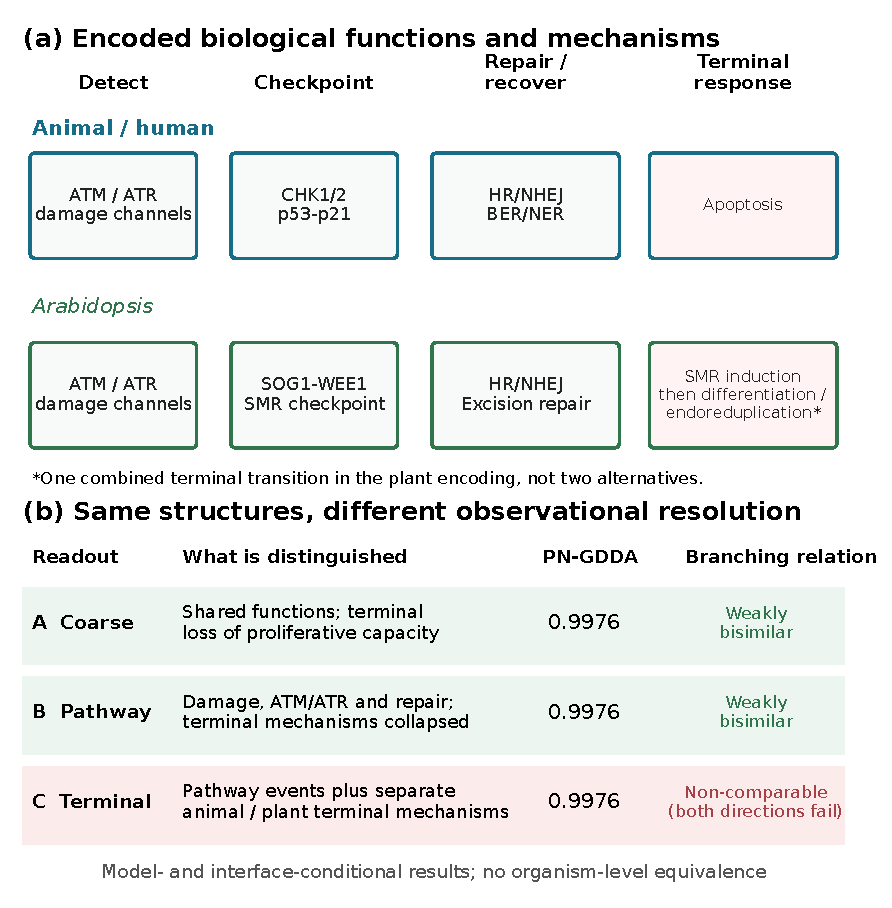
\includegraphics[width=\textwidth]{R2_Fig2.pdf}
\caption{Central GIM comparison. Upper-panel columns align encoded
animal/human and \tas{} functional categories; they are not a causal pathway
or a required sequence of outcomes. The lower panel
shows what each declared interface observes and the computed branching
relation. PN-GDDA remains 0.9976 because the structures are unchanged.
The combined plant terminal transition does not distinguish differentiation
from endoreduplication. Shared labels at A/B express a functional abstraction,
not identity between p53 and SOG1 or between terminal mechanisms.}
\label{fig:gim-interface}
\alttext{Animal and Arabidopsis damage-response functions above a three-row
interface comparison: A and B are weakly bisimilar; C is non-comparable,
with structural similarity constant at 0.9976.}
\end{figure}

\subsection{Coarse function retains correspondence}
At Interface A, every observable detection, checkpoint, repair, restoration,
or cycle-exit step in either executable model can be matched by the other,
with this matching preserved at the resulting states. Internal relays can
require different numbers of steps. Formally, the systems are weakly but not
strongly bisimilar. The result licenses comparison at the declared shared
functional level; it does not identify their molecular implementations.

\subsection{Pathway distinctions do not yet break the relation}
Interface B distinguishes damage channels, ATM/ATR-associated signaling, and
broad repair families. The models still match recursively when terminal
loss of proliferative capacity remains a common observation. Both simulation
directions and weak bisimilarity hold; strong bisimilarity does not.
Thus, among these encodings and interfaces, distinguishing those pathway
events alone is insufficient to eliminate the correspondence.

\subsection{Terminal mechanisms eliminate both directions}
At Interface C, mammalian \texttt{apoptosis} and plant
\texttt{smr\_induction} followed by
\texttt{differentiation\_or\_endoreduplication} become distinct observations.
Neither model can match all observable moves of the other, so weak
bisimilarity and both simulation directions fail. This is not an unexpected
biological discovery: the terminal labels intentionally encode prior knowledge
of different mechanisms. The computational result confirms where, in the
tested sequence of readouts, that distinction prevents recursive matching.
The depth-six trace distance becomes 0.3529 rather than zero; LTS-GDA changes
from 0.9508 to 0.8921. These diagnostics accompany the formal decision, not
replace it (Table~\ref{tab:gim-sensitivity}).

\begin{table}[t]
\tbl{Recomputed GIM results. Animal$\preceq$Plant means that the plant model
simulates the animal model; Plant$\preceq$Animal is the reverse.
Strong bisimilarity is false throughout.\label{tab:gim-sensitivity}}{
\begin{tabular}{@{}lccp{1.10in}rr@{}}
\toprule
Interface & Animal$\preceq$Plant & Plant$\preceq$Animal & Class & $d_6$ & PN-GDDA\\
\colrule
A: coarse & Y & Y & weak bisimulation & 0.0000 & 0.9976\\
B: pathway & Y & Y & weak bisimulation & 0.0000 & 0.9976\\
C: terminal & N & N & non-comparable & 0.3529 & 0.9976\\
\botrule
\end{tabular}}
\end{table}

\subsection{What changes when observability changes?}
Interfaces A and B aggregate terminal mechanisms into a shared functional
readout, whereas C separates them. The observed boundary is therefore
\emph{between B and C within this declared interface family}, not a uniquely
identified or globally minimal biological resolution. There is no exhaustive
search over all possible interfaces, and no experimental threshold is inferred.
The constant structural score isolates observability from topological change.

Prior biology supplies the distinct terminal mechanisms; PN-GDDA describes
their selected wiring; the executable comparison determines whether a
recursive correspondence survives each declared readout. Whether such a
model-level boundary predicts a cross-species experimental boundary remains
unvalidated. One testable interpretation is that readouts aggregating terminal
loss of proliferative capacity may preserve an apparent correspondence that
mechanism-specific readouts do not. This is a model-derived hypothesis, not an
assay result. The full Petri nets remain in \ref{app:gim-nets}.

\section{Supporting curated comparisons}\label{sec:case-method}

Five compact plant--animal pairs encode DNA repair/genome instability (GIM), energy
metabolism (DCE), cell-cycle control (SPS), cell death/autophagy (RCD), and
immune control (AID). Comparative studies and cancer-hallmark literature guided
component selection; dedicated reviews informed plant DNA-damage, cell-cycle,
and autophagy mechanisms.\cite{Quimbaya2012,ClavijoBuritica2023,Hanahan2022,
Yoshiyama2013} Transition-level provenance is machine-checked, which establishes
where encoded assumptions came from and whether documentation is complete. It
does not establish that the nets reproduce independent experiments. These
manually curated models contain no kinetics, concentrations, tissue context, or
independent experimental calibration.

The ten nets produced 5--14 reachable states. The GIM row in
Table~\ref{tab:case} reports Interface A; GIM, DCE, and SPS were weakly but
not strongly bisimilar; RCD gave plant-in-animal one-way simulation; AID was
non-comparable. Table~\ref{tab:case} juxtaposes these classes with native
PN-GDDA. The 592- and 576-orbit variants changed no score by 0.001 and no
threshold decision: all five pairs were structurally similar at 0.9 despite
three different behavioral classes.

\begin{table}[t]
\tbl{Supporting curated model-pair outputs. GIM is reported at Interface A;
all relations and $d_6$ values are interface-conditional, whereas PN-GDDA is
structural.\label{tab:case}}{
\begin{tabular}{@{}l>{\raggedright\arraybackslash}p{1.05in}>{\raggedright\arraybackslash}p{1.05in}rrr@{}}
\toprule
Module & Process & Formal class & $d_6$ & PN-592 & Orbit-576 \\
\colrule
GIM & DNA repair & weak bisimulation & 0.000 & 0.9976 & 0.9975 \\
DCE & energy metabolism & weak bisimulation & 0.000 & 0.9969 & 0.9968 \\
SPS & cell-cycle control & weak bisimulation & 0.000 & 1.0000 & 1.0000 \\
RCD & death/autophagy & plant in animal & 0.143 & 1.0000 & 1.0000 \\
AID & immune control & non-comparable & 0.429 & 0.9907 & 0.9904 \\
\botrule
\end{tabular}}
\end{table}

RCD supplies a secondary directional result: both encoded nets contain stress,
mTOR inhibition, autophagy, and survival, but only the animal encoding exposes a
canonical caspase-apoptosis branch; the plant branch uses an internal metacaspase
event. The plant LTS is weakly simulated by the animal LTS, whereas the reverse
direction fails. This means containment only for the declared labels of these
two models; it does not equate plant programmed cell death with mammalian
apoptosis. Silent subdivision preserved every class over 300 refinements per
module, while targeted relabeling changed the expected relations. Distances
against 2,000 label permutations assess internal interface sensitivity, not
external biological significance. DCE, SPS, and AID are retained as supporting
model-ingestion and relation-diversity examples rather than independent
biological validation.

\section{Exploratory confrontation with HPN-DREAM data}\label{sec:hpn-method}

An independent-data check is retained as a secondary, exploratory analysis,
not as validation of the GIM resolution boundary. Public HPN-DREAM/CASPOTS
families contain 72 BT20, 191 BT549, and 21 MCF7 Boolean networks.
Structure-only medoid selection, fixed before test-response access, chooses
zero-based rows 24, 137, and 9.\cite{Hill2016,Razzaq2018} The common interface
contains seven measured PI3K/MAPK/mTOR readouts under three shared held-out
mTOR-inhibitor conditions. Initial values, clamping, and update conventions
are specified in Supplementary Validation, Section~S3.

The nine asynchronous pair--condition comparisons contain six one-way
simulations and three non-comparable pairs. The six directions comprise three
left-model-in-right-model and three right-model-in-left-model relations, not
positions on an ordinal similarity scale. Direction is preserved in the result
fields; no scalar formal-class test is performed. Median profile RMSE is
0.2757, 0.1919, and 0.2071 in those three nominal categories, respectively,
with only three observations per category. Synchronous updating preserves
seven of the nine classes. These summaries cannot establish predictive value.

The retained continuous diagnostics are inconclusive: truncated-trace distance
has Spearman $\rho=-0.596$, exact one-sided $p=0.556$; LTS-GDA distance has
$\rho=0.669$, $p=0.097$, using all 216 condition-stratified permutations.
The CASPOTS native-context advantage over cross-cell medoids is 0.00212
excess-RMSE units and is not established by the exact three-cell sign test
($p=0.25$). No more favorable statistic was substituted. The full methods,
negative results, and plot remain in Supplementary Validation, Section~S3;
they show a route to data confrontation without claiming prognosis, native
cell-line specificity, or experimental equivalence.

\section{Supporting formal and implementation checks}
\label{sec:computational-validation}

Definitions and the executed relation-deletion method are supported by the
proofs in \ref{app:formal}. Table~\ref{tab:validation-summary} states
the checks, independent bases, and observed outcomes in the main article.
These checks address whether the implemented relations and structural score
behave as specified; they do not establish biological validity.

\begin{table}[!htbp]
\tbl{Main implementation-verification results. Agreement refers to the declared
inputs and predicates, not predictive accuracy on biological data.
\label{tab:validation-summary}}{
\small
\setlength{\tabcolsep}{4pt}
\renewcommand{\arraystretch}{1.08}
\begin{tabular}{@{}>{\raggedright\arraybackslash}p{0.205\textwidth}%
>{\raggedright\arraybackslash}p{0.37\textwidth}%
>{\raggedright\arraybackslash}p{0.37\textwidth}@{}}
\toprule
Check & Independent basis and scope & Observed result \\
\colrule
Constructed cases & Six pairs with classes fixed before classification & 6/6 classes and 6/6 binary weak-equivalence decisions recovered. \\
External equivalence & mCRL2 on six synthetic, six public-model controls, and nine HPN pairs & 42/42 strong/weak-bisimilarity decisions agree. \\
Directional audit & Raw-edge attacker--defender game on 32 model pairs and three hierarchy witnesses & No disagreement on either weak-simulation direction or strong/weak bisimilarity. \\
Exhaustive finite check & All 260 one-/two-state LTSs over $\{a,\tau\}$; 67,600 ordered pairs & No simulation or weak-bisimulation discrepancy; no hierarchy or trace-inclusion violation. \\
Structural score & Holmes 1.1.1: 151 graphlets, 592 slots; four-node net and one-arc-deletion control & PN-GDDA agrees to 12 decimal places; absolute difference $3.33\times10^{-16}$. \\
\botrule
\end{tabular}}
\end{table}

The public cell-cycle and p53--Mdm2 controls test SBML-qual and GINML imports;
all six copy, silent-refinement, and label-perturbation controls recover their
predeclared outcomes.\cite{Naldi2018,Chaouiya2013SBML,Traynard2016,AbouJaoude2009}
Holmes supplies an external reference for the PN-GDDA implementation.
\cite{Radom2017} mCRL2 supplies the external equivalence checks.
\cite{Bunte2019} Its simulation-preorder checks are used only for the two
tau-free hierarchy witnesses, where strong and weak simulation coincide;
no general weak-preorder verification is attributed to that tool.

For directional checks, the independent game constructs weak targets directly
from raw edges without calling the production closure or relation routines.
The 32 pairs comprise six synthetic, three GIM-interface, five curated, and
18 asynchronous/synchronous HPN comparisons. The exhaustive universe fixes
initial state zero and enumerates every edge subset; it is not a proof for
arbitrary finite systems. In particular, Example~\ref{ex:branching} separately
establishes early-to-late simulation, failure of the reverse, and exact trace
equality using an explicit witness and a failed-successor argument. No exact
trace conclusion is inferred from a truncated distance.

The evidence layers remain distinct: proofs establish mathematical claims;
tests establish implementation agreement on tested inputs; model provenance
and import checks establish executable assumptions; biological literature and
held-out data support or limit biological interpretation. Formal agreement alone
does not calibrate a curated net against experiments. Supplementary Validation
S1--S2 and S4 retain per-case outputs, comparator definitions, tool procedures,
and scaling details; the principal GIM evidence remains in Section~4.

\section{Discussion}\label{sec:discussion}

\subsection{What does structural similarity tell us?}
PN-GDDA describes similarity of local directed bipartite Petri-net wiring.
The GIM value 0.9976 is therefore meaningful but deliberately incomplete as a
statement about executable behavior. It remains constant when labels change
because the underlying structure does not. A label-blind score cannot determine
labeled trace equality or simulation in general (Proposition
\ref{prop:label-blind}); this is a boundary of the question it answers, not a
defect in the comparator. Structural and behavioral comparisons are
complementary, rather than competitors for one universal notion of similarity.

\subsection{What does behavioral comparison add?}
The executable comparison determines whether observable steps can be matched
recursively from the declared initial states. Unlike a trace list, it retains
the location at which choices become committed (Example~\ref{ex:branching}).
This distinction is relevant when transferring qualitative model behavior
requires preserving alternative continuations rather than merely permitting
the same sequences. Related formal work on asynchronous Boolean networks also
emphasizes reachable branching in phenotypic analysis.\cite{Yizengaw2026}

In GIM, the model-level answer is correspondence at A/B and its loss at C.
In RCD, only the plant model's declared branching behavior is reproducible by
the animal model, not conversely. Simulation is stronger than saying that
each plant trace occurs in the animal model: every related successor pair
must continue to satisfy the matching condition. Neither result transfers to
other interfaces or organisms without re-analysis.

\subsection{What does interface refinement mean biologically?}
An observational interface states which differences a biological readout is
allowed to retain, merge, or hide. At A/B, the GIM terminal responses are
collapsed into loss of proliferative capacity; at C, their encoded mechanisms
are distinguishable. Their incompatibility at C is consequently consistent
with the model construction, not independent evidence that the method has
discovered a new organism-level difference. The contribution is to determine
the survival or failure of recursive correspondence for the full executable
models under each explicit interface.

The result localizes a boundary within three declared readouts; it does not
optimize over interfaces or identify a unique minimal observational scale.
Because the interfaces were informed by known mechanisms, the C result is not
a blinded prediction. A prospective test would need independently selected
readouts, matched biological conditions, and outcomes not used in model or
interface construction. The present assay interpretation remains a hypothesis.
The distinction between a combined differentiation/endoreduplication transition
and two independently selectable outcomes is also essential: only the combined
transition is encoded here.

\subsection{Execution assumptions and evidence limits}
The comparison depends on transitions, initial states, labels, and update
semantics, not on graph structure alone. Asynchronous versus synchronous
execution changes public-model reachability and two HPN classes. General
asynchronous, most-permissive, and stochastic semantics were not evaluated.
\cite{Pauleve2020} Weak bisimulation here is divergence-insensitive and concerns
untimed interleaving behavior, not rates, probabilities, or true concurrency.
Controlled silent refinement preserves the relation only under the stated
construction (Proposition~\ref{prop:silent-refinement}), not under arbitrary
insertions of conflicts or observable branches.

The GIM pair is manually curated and compact, with no kinetics, concentrations,
tissue context, or independent experimental calibration. Literature justifies
the chosen biological distinctions but does not certify the entire executable
model. HPN provides independent measurements yet has only nine pair--condition
observations, three cell lines, and inconclusive associations. Its formal
directions are nominal; assigning them an ordinal score would lose information.
CASPOTS RMSE is minimum-distance compatibility over admissible trajectories,
not a unique time-series prediction. These limitations cannot be removed by
adding more software controls.

\subsection{Computational scope}
Explicit reachability remains vulnerable to state-space explosion, and a
candidate relation stores the product of the two state sets. The scaling study
in Supplementary Validation is illustrative, not evidence of genome-scale
performance. Applying native PN-GDDA to logical rules would additionally require
a non-unique Petri-net translation. Larger independently curated model pairs,
prospectively chosen interfaces, and empirical readouts are needed before
claiming wider biological utility. The present method is most defensible as a
reproducible, question-specific comparison of explicit qualitative models.

\section{Conclusion}\label{sec:conclusion}

Two curated DNA-damage response models with constant PN-GDDA similarity 0.9976
retain recursive behavioral correspondence at coarse and pathway resolution,
but become non-comparable when their encoded terminal mechanisms are separately
observed. For these models, correspondence depends on observational resolution;
the boundary lies between Interfaces B and C within the declared family.

The computational contribution is to make that conditional boundary explicit
and reproducible, while preserving the difference between similar wiring,
matching traces, and matching branching. Proofs and independent checks support
the formal decisions without substituting for biological evidence. The result
does not establish organism-level equivalence, mechanistic identity, or
prognosis. Its empirical relevance remains to be tested beyond these curated
models; the secondary HPN analysis is exploratory and inconclusive.

\appendix
\section{Mathematical properties and quantifier audit}\label{app:formal}
\label{sec:fixed-point}

For $a\in\Sigma_{\TAU}$, let $D_a^i(x)=\{x':x\xrightarrow{a}_i x'\}$ and
$U=S_1\times S_2$. Define operators on $\powerset(U)$ by
\begin{align}
\Phi_{\preceq}(R)=\{(x,y)\in U:
 &\ \forall a,x'\in D_a^1(x)\ \exists y'\in W_a^2(y),
 (x',y')\in R\},\label{eq:sim-operator}\\
\Phi_w(R)=\{(x,y)\in\Phi_{\preceq}(R):
 &\ \forall a,y'\in D_a^2(y)\ \exists x'\in W_a^1(x),
 (x',y')\in R\},\label{eq:weak-bisim-operator}\\
\Phi_s(R)=\{(x,y)\in U:
 &\ \forall a,x'\in D_a^1(x)\ \exists y'\in D_a^2(y),
 (x',y')\in R,\nonumber\\
 &\ \forall a,y'\in D_a^2(y)\ \exists x'\in D_a^1(x),
 (x',y')\in R\}.\label{eq:strong-bisim-operator}
\end{align}

\begin{theorem}[Correctness of relation deletion]\label{thm:fixed-point}
For each $\Phi\in\{\Phi_{\preceq},\Phi_w,\Phi_s\}$, the operator is monotone.
The implemented algorithm starts with $R=U$, repeatedly deletes any currently
examined pair $z\notin\Phi(R)$, and stops after a complete pass with no deletion.
On finite LTSs it terminates and returns the greatest fixed point $\nu\Phi$.
Consequently, testing membership of $(s_1^0,s_2^0)$ computes, respectively,
weak simulation in the orientation of Definition \ref{def:weak-simulation}, weak
bisimilarity, and strong bisimilarity.
\end{theorem}

\begin{proof}
If $R\subseteq Q$, every witness pair in $R$ remains available in $Q$; hence
$\Phi(R)\subseteq\Phi(Q)$ for each operator. Every deletion strictly decreases
the finite relation, so termination requires at most $|U|$ deletions.

Let $G=\nu\Phi$. The invariant $G\subseteq R$ holds initially. If it holds before
a deletion and $z\in G$, then
$z\in\Phi(G)\subseteq\Phi(R)$, so $z$ cannot be deleted. Thus $G$ remains a
subset of the terminal relation $R_*$. A final pass without deletion gives
$R_*\subseteq\Phi(R_*)$. Conversely, each $z\notin R_*$ was deleted from some
$R_z$ with $z\notin\Phi(R_z)$. Since $R_*\subseteq R_z$, monotonicity implies
$\Phi(R_*)\subseteq\Phi(R_z)$ and therefore $z\notin\Phi(R_*)$. Hence
$R_*=\Phi(R_*)$. Because $R_*$ is a fixed point, $R_*\subseteq G$; together
with the invariant this yields $R_*=G$. The three operators are exactly the
transfer clauses of Definitions \ref{def:weak-simulation} and
\ref{def:bisimulation}.
\end{proof}

\begin{remark}[Resource bound]\label{rem:complexity}
Writing $n_i=|S_i|$, the candidate relation stores $O(n_1n_2)$ pairs and permits
at most $n_1n_2$ deletions and $n_1n_2+1$ passes. Each pass scans current pairs,
outgoing moves, and matching direct or weak targets. Silent closures are cached;
visible weak targets are constructed on demand. We therefore report these
parameters instead of claiming an unjustified tight time bound.
\end{remark}

\begin{proposition}[Hierarchy of behavioral relations]\label{prop:hierarchy}
For finite LTSs under Definitions \ref{def:weak-move}--\ref{def:weak-traces},
\begin{equation}\label{eq:hierarchy}
L_1\strongsim L_2
\Longrightarrow L_1\weaksim L_2
\Longrightarrow
(L_1\weakpre L_2\ \land\ L_2\weakpre L_1)
\Longrightarrow L_w(L_1)=L_w(L_2).
\end{equation}
The converses do not hold in general.
\end{proposition}

\begin{proof}
A direct match is a permitted weak match, and each direction of a weak
bisimulation is a weak simulation. If $L_1\weakpre L_2$, induction along any
finite concrete path matches observable moves by $\TAU^*a\TAU^*$ and silent
moves by $\TAU^*$, preserving related successors. Erasing $\TAU$ gives
$L_w(L_1)\subseteq L_w(L_2)$; the reverse simulation gives equality.
Proposition \ref{prop:silent-refinement} and Example \ref{ex:branching} refute
the first and last converses. For the middle converse, compare
$a.(b+c)+a.b$ with $a.(b+c)$: each simulates the other, but the $a.b$ successor
cannot be bisimilar to a state offering both $b$ and $c$.
\end{proof}


\begin{table}[t]
\tbl{Distinct witnesses for the three failed converses. All pairs have equal
exact weak-trace languages; $X\preceq Y$ means $Y$ simulates $X$.
\label{tab:hierarchy-witnesses}}{
\begin{tabular}{@{}p{1.75in}p{1.6in}p{1.3in}@{}}
\toprule
Converse refuted & Witness pair $(X,Y)$ & Decisive properties\\
\colrule
Weak implies strong bisimilarity & $a.0$, $a.\tau.0$ & weak, not strong\\
Mutual simulation implies weak bisimilarity & $a.(b+c)+a.b$, $a.(b+c)$ & both directions, not weak\\
Exact trace equality implies mutual simulation & late choice, early choice & early$\preceq$late only\\
\botrule
\end{tabular}}
\end{table}

For the middle row, write $x_{bc},x_b$ for the two $a$-successors of $X$ and
$y_{bc}$ for the sole $a$-successor of $Y$. A simulation from $X$ to $Y$
relates both $x_{bc}$ and $x_b$ to $y_{bc}$, with corresponding terminal
pairs. A simulation from $Y$ to $X$ relates $y_{bc}$ only to $x_{bc}$.
Both initial pairs therefore survive. A bisimulation would additionally need
to match $X$'s transition to $x_b$ with $y_{bc}$; the latter's $c$-move has
no counterpart at $x_b$. This witness concerns only the middle converse,
not the trace-equality converse refuted by Example~\ref{ex:branching}.

\begin{proposition}[Controlled silent edge refinement]
\label{prop:silent-refinement}
Let $L$ contain $p\xrightarrow{a}q$ with $a\in\Sigma$ and $p\neq q$. Construct
$L'$ by copying all original states and transitions except this edge, and replacing
it by
\begin{equation}\label{eq:silent-refinement}
 \bar p\xrightarrow{a}r\xrightarrow{\TAU}\bar q,
\end{equation}
where $r$ is fresh and has no other incident behavior. Then $L\weaksim L'$.
Repeated refinements of this form also preserve weak bisimilarity. If $p$ and
$\bar p$ are initial, the selected edge is the only $a$-edge from $\bar p$ in
$L'$, and every $a$-successor of $p$ in $L$ has no outgoing $\TAU$ transition,
then $L\not\strongsim L'$.
\end{proposition}

\begin{proof}
Let
$R=\{(x,\bar x):x\in S\}\cup\{(q,r)\}$. For every copied pair other than the
source, direct moves are copied. At $(p,\bar p)$, the original edge is matched
by $\bar p\xrightarrow{a}r\xrightarrow{\TAU}\bar q$, while
$\bar p\xrightarrow{a}r$ is matched by $p\xrightarrow{a}q$ and ends in
$(q,r)$. At $(q,r)$, moves from $q$ are matched after
$r\xrightarrow{\TAU}\bar q$; that silent move is itself matched by zero silent
moves at $q$. Hence $R$ is a weak bisimulation, and repetition follows by
transitivity. Under the additional conditions, a strong match for
$\bar p\xrightarrow{a}r$ must relate $r$ to an $a$-successor $x$ of $p$, but
$r\xrightarrow{\TAU}\bar q$ would require the excluded direct $\TAU$-move from
$x$. Thus strong bisimilarity fails.
\end{proof}

\begin{proposition}[Limit of label-blind structural comparison]
\label{prop:label-blind}
Let $M$ be any comparator determined only by unlabeled structure and invariant
under relabeling of transitions. Then $M$ cannot characterize weak-trace
equality, weak simulation or weak bisimilarity for labeled systems in general.
\end{proposition}

\begin{proof}
Take two systems with the same two states and one directed edge. Label the edge
$a$ in $L_a$ and $b\neq a$ in $L_b$. Their unlabeled structures are identical,
so $M(L_a,L_b)=M(L_a,L_a)$. Yet their languages are
$\{\epsilon,a\}$ and $\{\epsilon,b\}$, and neither observable move can be
matched by the other system. Thus no decision based only on $M$ can characterize
the stated labeled relations.
\end{proof}

Proposition \ref{prop:label-blind} does not identify a defect in PN-GDDA. It
states that a label-blind structural method answers a different question and
cannot substitute for a labeled behavioral relation.

\begin{example}[Equal traces, different branching]\label{ex:branching}
Let the late-choice system start at $\ell_0$ and have exactly
\begin{equation}\label{eq:late-choice}
\ell_0\xrightarrow{a}\ell_1,\qquad
\ell_1\xrightarrow{b}\ell_b,\qquad \ell_1\xrightarrow{c}\ell_c,
\end{equation}
and let the early-choice system start at $e_0$ and have exactly
\begin{equation}\label{eq:early-choice}
e_0\xrightarrow{a}e_b,\quad e_0\xrightarrow{a}e_c,\quad
e_b\xrightarrow{b}e'_b,\quad e_c\xrightarrow{c}e'_c.
\end{equation}
All unlisted states are terminal; neither system has silent transitions or
cycles. Enumerating all paths, whose lengths are at most two, gives both exact
prefix-closed languages as $\{\epsilon,a,ab,ac\}$, not merely a truncated match.

An explicit simulation from early to late is
\begin{equation}\label{eq:early-late-witness}
R_{E\to L}=\{(e_0,\ell_0),(e_b,\ell_1),(e_c,\ell_1),
(e'_b,\ell_b),(e'_c,\ell_c)\}.
\end{equation}
Both initial $a$-moves are matched by $\ell_0\xrightarrow{a}\ell_1$.
At $(e_b,\ell_1)$ the sole $b$-move has a match; at $(e_c,\ell_1)$ the sole
$c$-move has a match. Terminal pairs impose no further obligations. Thus
$L_{\mathrm{early}}\weakpre L_{\mathrm{late}}$.

Conversely, suppose a simulation $R$ from late to early contains
$(\ell_0,e_0)$. Matching the single transition
$\ell_0\xrightarrow{a}\ell_1$ requires choosing one successor of $e_0$ and
including the resulting pair in $R$. If $(\ell_1,e_b)\in R$, the $c$-move
from $\ell_1$ has no match. If $(\ell_1,e_c)\in R$, its $b$-move has no
match. These exhaust the possible $a$-successors, so no such $R$ exists:
$L_{\mathrm{late}}\not\weakpre L_{\mathrm{early}}$. Weak bisimilarity
therefore also fails.

Different outgoing transitions from a related pair may indeed choose different
matching successors. However, the \emph{one} initial late $a$-transition must
be matched by an early successor pair that itself satisfies every subsequent
transfer obligation. Trace matching may select the $e_b$ branch for $ab$ and
the $e_c$ branch for $ac$ independently; simulation cannot combine those two
states into one defender state after the initial move. This is the quantifier
distinction behind the final strictness claim of Proposition
\ref{prop:hierarchy}.
\end{example}

\section{Detailed GIM Petri-net encodings}\label{app:gim-nets}

Figures~\ref{fig:gim-animal-net} and \ref{fig:gim-plant-net} show the
fixed executable nets; the three interfaces change only transition labels.

\clearpage
\begin{sidewaysfigure}[p]
\centering
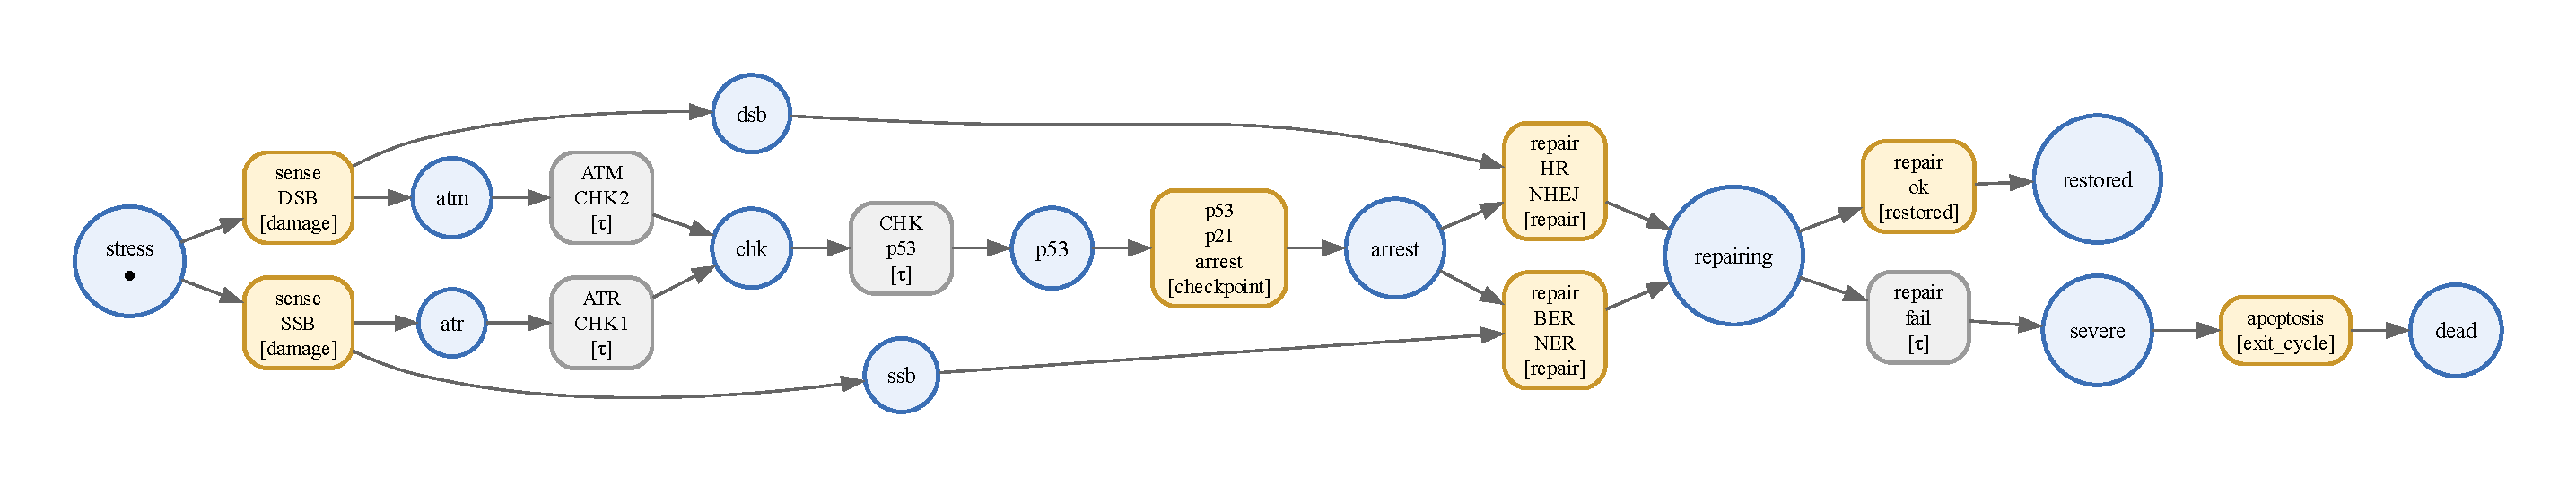
\includegraphics[width=0.94\textheight]{R2_Fig3.pdf}
\caption{Detailed animal/human GIM Petri net. Circles are places, rounded boxes
are transitions, brackets show the base/coarse observable labels, and gray
$\tau$ transitions are internal.}
\label{fig:gim-animal-net}
\alttext{Detailed animal and human DNA-damage Petri net with places,
transitions, labels, and arcs.}
\end{sidewaysfigure}

\begin{sidewaysfigure}[p]
\centering
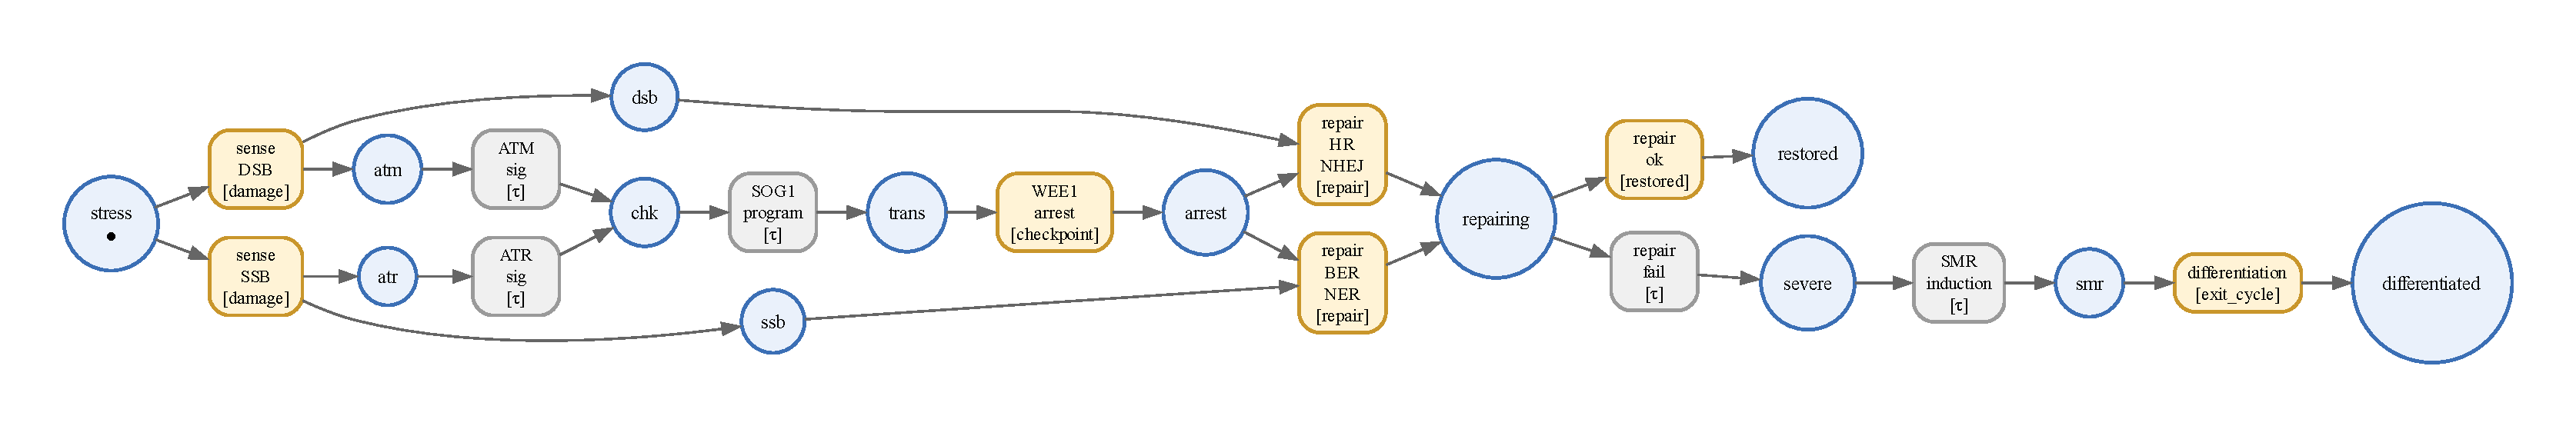
\includegraphics[width=0.94\textheight]{R2_Fig4.pdf}
\caption{Detailed \tas{} GIM Petri net, using the same graphical conventions as
Fig.~\ref{fig:gim-animal-net}. The terminal transition is a combined outcome in
this encoding and does not distinguish differentiation from endoreduplication.}
\label{fig:gim-plant-net}
\alttext{Detailed Arabidopsis DNA-damage Petri net with places, transitions,
labels, and arcs.}
\end{sidewaysfigure}

\clearpage

\section*{Data and code availability}

Code, curated definitions, hash-verified public models, normalized response
files, metadata, and generated results are available under the MIT License at
\url{https://github.com/cero1979/BisimulationMol}. The second-revision source and audits are in \texttt{revision\_R2/}.
The repository documents
formal/software verification, interface definitions, figure regeneration,
tests, and notebook execution. Machine-readable GIM and HPN results are provided
as \texttt{results/gim\_interface\_sensitivity.csv} and
\texttt{results/hpn\_dream\_formal\_data\_validation.csv}. No confidential or
participant-level data were used.

\section*{Declarations}

\noindent\textbf{Funding.} No specific funding was received.
\textbf{Competing interests.} The author declares no competing interests.
\textbf{Ethics.} Only computational models and published aggregate data were
used; no human participants, samples, or live animals were involved.
\textbf{Author contributions.} Carlos Ramirez Ovalle performed the
conceptualization, methodology, software, formal analysis, validation,
visualization, drafting, and revision.

\begin{thebibliography}{10}
\providecommand{\url}[1]{\texttt{#1}}
\providecommand{\urlprefix}{URL }
\expandafter\ifx\csname urlstyle\endcsname\relax
  \providecommand{\doi}[1]{doi:\discretionary{}{}{}#1}\else
  \providecommand{\doi}{doi:\discretionary{}{}{}\begingroup
  \urlstyle{rm}\Url}\fi

\bibitem{ChaouiyaPetriBio2007}
Chaouiya C, Petri net modelling of biological networks, \emph{Briefings in
  Bioinformatics} \textbf{8}(4):210--219, 2007.
\newblock \doi{10.1093/bib/bbm029}.

\bibitem{Li2006}
Li C, Suzuki S, Ge QW, Nakata M, Matsuno H, Miyano S, Structural modeling and
  analysis of signaling pathways based on {Petri} nets, \emph{Journal of
  Bioinformatics and Computational Biology} \textbf{4}(5):1119--1140, 2006.
\newblock \doi{10.1142/S021972000600234X}.

\bibitem{Fisher2007}
Fisher J, Henzinger TA, Executable cell biology, \emph{Nature Biotechnology}
  \textbf{25}(11):1239--1249, 2007.
\newblock \doi{10.1038/nbt1356}.

\bibitem{JacksonBartek2009}
Jackson SP, Bartek J, The {DNA}-damage response in human biology and disease,
  \emph{Nature} \textbf{461}(7267):1071--1078, 2009.
\newblock \doi{10.1038/nature08467}.

\bibitem{BlackfordJackson2017}
Blackford AN, Jackson SP, {ATM}, {ATR}, and {DNA-PK}: The trinity at the heart
  of the {DNA} damage response, \emph{Molecular Cell} \textbf{66}(6):801--817,
  2017.
\newblock \doi{10.1016/j.molcel.2017.05.015}.

\bibitem{Yoshiyama2013}
Yoshiyama KO, Sakaguchi K, Kimura S, Dna damage response in plants: conserved
  and variable response compared to animals, \emph{Biology}
  \textbf{2}(4):1338--1356, 2013.
\newblock \doi{10.3390/biology2041338}.

\bibitem{DeSchutter2007}
De~Schutter K, Joub{\`e}s J, Cools T, Verkest A, Corellou F, Babiychuk E, Van
  Der~Schueren E, Beeckman T, Kushnir S, Inz{\'e} D, De~Veylder L,
  {Arabidopsis} {WEE1} kinase controls cell cycle arrest in response to
  activation of the {DNA} integrity checkpoint, \emph{The Plant Cell}
  \textbf{19}(1):211--225, 2007.
\newblock \doi{10.1105/tpc.106.045047}.

\bibitem{Yi2014}
Yi D, Kamei CLA, Cools T, Vanderauwera S, Takahashi N, Okushima Y, Eekhout T,
  Yoshiyama KO, \emph{et~al.}, The {Arabidopsis} {SIAMESE-RELATED}
  cyclin-dependent kinase inhibitors {SMR5} and {SMR7} regulate the {DNA}
  damage checkpoint in response to reactive oxygen species, \emph{The Plant
  Cell} \textbf{26}(1):296--309, 2014.
\newblock \doi{10.1105/tpc.113.118943}.

\bibitem{Adachi2011}
Adachi S, Minamisawa K, Okushima Y, Inagaki S, Yoshiyama K, Kondou Y, Kaminuma
  E, Kawashima M, Toyoda T, Matsui M, Kurihara D, Matsunaga S, Umeda M,
  Programmed induction of endoreduplication by {DNA} double-strand breaks in
  {Arabidopsis}, \emph{Proceedings of the National Academy of Sciences}
  \textbf{108}(24):10004--10009, 2011.
\newblock \doi{10.1073/pnas.1103584108}.

\bibitem{Szawulak2022}
Szawulak B, Formanowicz P, Graphlets in comparison of {Petri} net-based models
  of biological systems, \emph{Scientific Reports} \textbf{12}:20942, 2022.
\newblock \doi{10.1038/s41598-022-24535-5}.

\bibitem{Milner1989}
Milner R, \emph{Communication and Concurrency}, Prentice Hall, New York, 1989.
\newblock ISBN 978-0-13-115007-2.

\bibitem{Sangiorgi2011}
Sangiorgi D, \emph{Introduction to Bisimulation and Coinduction}, Cambridge
  University Press, Cambridge, 2011.
\newblock ISBN 978-1-107-00363-7.
\newblock \doi{10.1017/CBO9780511777110}.

\bibitem{Hill2016}
Hill SM, Heiser LM, Cokelaer T, Unger M, Nesser NK, Carlin DE, \emph{et~al.},
  Inferring causal molecular networks: Empirical assessment through a
  community-based effort, \emph{Nature Methods} \textbf{13}(4):310--318, 2016.
\newblock \doi{10.1038/nmeth.3773}.

\bibitem{Razzaq2018}
Razzaq M, Paulev{\'e} L, Siegel A, Saez-Rodriguez J, Bourdon J, Guziolowski C,
  Computational discovery of dynamic cell line specific boolean networks from
  multiplex time-course data, \emph{PLOS Computational Biology}
  \textbf{14}(10):e1006538, 2018.
\newblock \doi{10.1371/journal.pcbi.1006538}.

\bibitem{Ogita2018}
Ogita N, Okushima Y, Tokizawa M, Yamamoto YY, Tanaka M, Seki M, Makita Y,
  Matsui M, Okamoto-Yoshiyama K, \emph{et~al.}, Identifying the target genes of
  {SUPPRESSOR OF GAMMA RESPONSE 1}, a master transcription factor controlling
  {DNA} damage response in {Arabidopsis}, \emph{The Plant Journal}
  \textbf{94}(3):439--453, 2018.
\newblock \doi{10.1111/tpj.13866}.

\bibitem{ManovaGruszka2015}
Manova V, Gruszka D, {DNA} damage and repair in plants---from models to crops,
  \emph{Frontiers in Plant Science} \textbf{6}:885, 2015.
\newblock \doi{10.3389/fpls.2015.00885}.

\bibitem{FulcherSablowski2009}
Fulcher N, Sablowski R, Hypersensitivity to {DNA} damage in plant stem cell
  niches, \emph{Proceedings of the National Academy of Sciences}
  \textbf{106}(49):20984--20988, 2009.
\newblock \doi{10.1073/pnas.0909218106}.

\bibitem{Murata1989}
Murata T, Petri nets: Properties, analysis and applications, \emph{Proceedings
  of the IEEE} \textbf{77}(4):541--580, 1989.
\newblock \doi{10.1109/5.24143}.

\bibitem{Quimbaya2012}
Quimbaya M, Vandepoele K, Rasp{\'e} E, Matthijs M, Dhondt S, Beemster GTS, Berx
  G, De~Veylder L, Identification of putative cancer genes through data
  integration and comparative genomics between plants and humans,
  \emph{Cellular and Molecular Life Sciences} \textbf{69}(12):2041--2055, 2012.
\newblock \doi{10.1007/s00018-011-0909-x}.

\bibitem{ClavijoBuritica2023}
Clavijo-Buritic\'a DC, Sosa CC, C\'ardenas-Heredia R, Mosquera AJ, \'Alvarez A,
  Medina J, Quimbaya M, Use of {Arabidopsis thaliana} as a model to understand
  specific carcinogenic events: Comparison of the molecular machinery
  associated with cancer-hallmarks in plants and humans, \emph{Heliyon}
  \textbf{9}(4):e15367, 2023.
\newblock \doi{10.1016/j.heliyon.2023.e15367}.

\bibitem{Hanahan2022}
Hanahan D, Hallmarks of cancer: new dimensions, \emph{Cancer Discovery}
  \textbf{12}(1):31--46, 2022.
\newblock \doi{10.1158/2159-8290.CD-21-1059}.

\bibitem{Naldi2018}
Naldi A, Hernandez C, Abou-Jaoud\'e W, Monteiro PT, Chaouiya C, Thieffry D,
  Logical modeling and analysis of cellular regulatory networks with {GINsim}
  3.0, \emph{Frontiers in Physiology} \textbf{9}:646, 2018.
\newblock \doi{10.3389/fphys.2018.00646}.

\bibitem{Chaouiya2013SBML}
Chaouiya C, B\'erenguier D, Keating SM, Naldi A, van Iersel MP, Rodriguez N,
  \emph{et~al.}, {SBML} qualitative models: a model representation format and
  infrastructure to foster interactions between qualitative modelling
  formalisms and tools, \emph{BMC Systems Biology} \textbf{7}:135, 2013.
\newblock \doi{10.1186/1752-0509-7-135}.

\bibitem{Traynard2016}
Traynard P, Faur\'e A, Fages F, Thieffry D, Logical model specification aided
  by model-checking techniques: Application to the mammalian cell cycle
  regulation, \emph{Bioinformatics} \textbf{32}(17):i772--i780, 2016.
\newblock \doi{10.1093/bioinformatics/btw457}.

\bibitem{AbouJaoude2009}
Abou-Jaoud\'e W, Ouattara DA, Kaufman M, From structure to dynamics: Frequency
  tuning in the p53--mdm2 network, \emph{Journal of Theoretical Biology}
  \textbf{258}(4):561--577, 2009.
\newblock \doi{10.1016/j.jtbi.2009.02.005}.

\bibitem{Radom2017}
Radom M, Rybarczyk A, Szawulak B, Andrzejewski H, Chabelski P, Kozak A,
  Formanowicz P, Holmes: A graphical tool for development, simulation and
  analysis of {Petri} net based models of complex biological systems,
  \emph{Bioinformatics} \textbf{33}(23):3822--3823, 2017.
\newblock \doi{10.1093/bioinformatics/btx492}.

\bibitem{Bunte2019}
Bunte O, Groote JF, Keiren JJA, Laveaux M, Neele T, de~Vink EP, Wesselink W,
  Wijs A, Willemse TAC, The {mCRL2} toolset for analysing concurrent systems:
  Improvements in expressivity and usability,  \emph{Tools and Algorithms for
  the Construction and Analysis of Systems (TACAS 2019)}, Lecture Notes in
  Computer Science, Vol.~11428, Springer, pp. 21--39, 2019.
\newblock \doi{10.1007/978-3-030-17465-1_2}.

\bibitem{Yizengaw2026}
Yizengaw BY, Trap spaces as labelled ideals of {SCC} posets: A
  structural--functional theory of reachability in asynchronous {Boolean}
  networks, \emph{Journal of Bioinformatics and Computational Biology}
  \textbf{24}(3):2650007, 2026.
\newblock \doi{10.1142/S0219720026500071}.

\bibitem{Pauleve2020}
Paulev{\'e} L, Kol{\v{c}}{\'a}k J, Chatain T, Haar S, Reconciling qualitative,
  abstract, and scalable modeling of biological networks, \emph{Nature
  Communications} \textbf{11}:4256, 2020.
\newblock \doi{10.1038/s41467-020-18112-5}.

\end{thebibliography}

\end{document}
